\documentclass[letterpaper, 10 pt, conference,onecolumn]{ieeeconf}  % Comment this line out if you need a4paper

%\documentclass[a4paper, 10pt, conference]{ieeeconf}      % Use this line for a4 paper


\usepackage{cite}
\usepackage{epsfig}
\usepackage{epstopdf}
\usepackage[cmex10]{amsmath}
\usepackage{amssymb}
\usepackage{array}
\usepackage{mdwmath}
\usepackage{mdwtab}
\usepackage{cases}
\usepackage{eqparbox}
\usepackage{subfig}
\usepackage{color}
\usepackage{pifont}
\usepackage{tikz}
\definecolor{brown}{rgb}{0.823529 ,0.411765, 0.117647}
%\usepackage[usenames,dvipsnames]{color}
%\usepackage{ulem}

\IEEEoverridecommandlockouts
% This command is only needed if% you want to use the \thanks command

\overrideIEEEmargins                                      % Needed to meet printer requirements.

% See the \addtolength command later in the file to balance the column lengths
% on the last page of the document

% The following packages can be found on http:\\www.ctan.org
%\usepackage{graphics} % for pdf, bitmapped graphics files
%\usepackage{epsfig} % for postscript graphics files
%\usepackage{mathptmx} % assumes new font selection scheme installed
%\usepackage{times} % assumes new font selection scheme installed
%\usepackage{amsmath} % assumes amsmath package installed
%\usepackage{amssymb}  % assumes amsmath package installed

%\title{\LARGE \bf
%Distributed $\varepsilon$-Nash Strategies for Multi-Agent Formation Control}
%
%
%\author{Wei~Lin$^\dag$,~\IEEEmembership{Student Member,~IEEE,}
%        Zhihua~Qu$^\dag$,~\IEEEmembership{Fellow,~IEEE,}
%        and~Marwan~A. Simaan$^\dag$,~\IEEEmembership{Life Fellow,~IEEE}
%% <-this % stops a space
%\thanks{*This work is supported in part by US National Science Foundation under grants ECCS-1308928 and CCF-0956501 as well as by US Department of Energy's award DE-EE0006340 under the Grid Engineering for Accelerated Renewable Energy Deployment (GEARED) program and another subcontract under the Solar Energy Grid Integration Systems (SEGIS) program (phases I to III).}% <-this % stops a space
%\thanks{$^\dag$Wei Lin, Zhihua Qu, and Marwan A. Simaan are with the Department of EECS, University of Central Florida, Orlando, Florida, 32816, USA. Emails:
%        {\tt\small weilin0929@gmail.com, qu@eecs.ucf.edu, simaan@eecs.ucf.edu}.}%
%%
%}

\begin{document}
\title{\LARGE \bf
Distributed Game Strategy Design with Application to Multi-Agent Formation Control}


\author{Wei~Lin,~\IEEEmembership{Member,~IEEE,}
        Zhihua~Qu,~\IEEEmembership{Fellow,~IEEE,},~and
        Marwan~A. Simaan,~\IEEEmembership{Life Fellow,~IEEE}
% <-this % stops a space
\thanks{This work is supported in part by US National Science Foundation under grants ECCS-1308928 and CCF-0956501, by US Department of Energy¡¯s award DE-EE0006340, by US Department of Transportation¡¯s award DTRT13-G-UTC51, by L-3 Communication¡¯s contract 11013I2034, and by Leidos¡¯ contract P010161530.}% <-this % stops a space
\thanks{Wei Lin received his PhD degree from University of Central Florida in Dec. 2013 and is currently working in Western Digital Corporation, Irvine, CA, 92612, USA. E-mail: weilin0929@gmail.com.}
\thanks{Zhihua Qu and Marwan A. Simaan are with the Department of EECS, University of Central Florida, Orlando, Florida, 32816, USA, e-mails: qu@eecs.ucf.edu, simaan@eecs.ucf.edu.}%
%
}


%\markboth{Journal of \LaTeX\ Class Files,~Vol.~11, No.~4, December~2012}%
%{Shell \MakeLowercase{\textit{et al.}}: Bare Demo of IEEEtran.cls for Journals}

\maketitle

\IEEEpeerreviewmaketitle

%%%%%%%%%%%%%%%%%%%%%%%%%%%%%%%%%%%%%%%%%%%%%%%%%%%%%%%%%%%%%%%%%%%%%%%%%%%%%%%%
\begin{abstract}
In this paper, we consider {a} multi-agent formation control problem from {a} game {theory} point of view. It is well known that a major difficulty in a communication network based formation control problem is that each agent is only able to exchange information {with other agents} according to the communication topology. This information constraint prevents many game strategy design approaches that require individual agents to have global information from being implemented in many cases. We formulate the formation control problem {in such a way that individual agents try to minimize their locally measured formation errors and {to} solve it as a differential game problem}. We consider two cases of non-cooperative and cooperative games and {propose} a novel distributed design approach that utilizes the relationship between the initial and terminal state variables. This approach is applied to an illustrative formation control example among three agents and the formation errors under various scenarios are compared and analyzed.
\end{abstract}

\newtheorem{Def}{Definition}
\newtheorem{Asu}{Assumption}
\newtheorem{thm}{Theorem}
\newtheorem{Pro}{Proposition}
\newtheorem{Alg}{Algorithm}
\newtheorem{Lem}{Lemma}
\newtheorem{Rmk}{Remark}


\section{Introduction}
{An} important application of cooperative control theory \cite{ren,Qu} {is} the multi-agent formation control problems \cite{Stipanovic2004,Keviczky2008,JiananWang2012}. {This problem revolves around designing} local information constrained control inputs for the agents (mobile robots, unmanned vehicles, etc) and {making} their positions {follow} a prescribed formation. There {is considerable work} done in this field and the comprehensive review paper \cite{Cao2013} on multi-agent distributed control systems is a good reference on {recent} progress {in} cooperative control theory including the formation control problem. Recently, multiple attempts \cite{anderson1998formation,DongbingGu2008,SemsarKazerooni20092205} have been made to incorporate {differential} game theory \cite{Isaacs,Basar} into the formation control design problem. {A fundamental connection {between these two problems} can be explained as follows: in a multi-agent formation control problem, all the agents are basically trying to minimize the formation errors between each other. If every agent is able to observe all the other agents, then the problem can be essentially viewed as an optimal control problem where a common performance index of global formation errors can be assigned for all the agents. However, in most of {realistic} applications,} since the agents are usually connected through {a} communication network {with} a certain topology, they are only able to exchange information with each other in a distributed manner (i.e., to share information locally). {In {this} case, instead of minimizing a globally defined performance index, it is {more realistic} for each agent to only minimize a performance index of its locally measured formation errors. This scenario is exactly equivalent to that of a differential game where each player is trying to minimize its own performance index. Therefore, most {multi-agent} formation control design {problems} can be viewed and solved as {differential game problems}. The game solutions including {Nash equilibria} for non-cooperative agents and Pareto optimality for cooperative agents can {be} well established. However, solving {for} the Nash and Pareto solutions under distributed information is not a trivial task in the multi-agent environment because of the following two {issues}: (1) the strategy for each agent has to conform to its local information topology constraint and (2) local strategy computing within each agent is preferred rather than centralized strategy computing where strategies are designed by a centralized designer and assigned to individual agents.} In \cite{DongbingGu2008,SemsarKazerooni20092205}, the first {issue} has been addressed and the corresponding Nash and Pareto strategies are considered for the formation control problem as a differential game. {In} this present paper, we will focus more on the second aspect. By investigating the structure of the game solution in more details, a strategy design approach as well as {an} implementation algorithm {are} proposed for each agent to carry out its optimal control strategy design in a fully distributed manner. The {remainder} of this paper is organized as follows. A brief setup of the game {problem} is presented in Section \ref{setup}. The main results of the distributed Nash and Pareto strategy {designs} are presented in Section \ref{mainresult1} and \ref{mainresult2} {respectively}. An illustrative example with three agents under noncooperative and cooperative cases is presented and analyzed in Section \ref{simulation}.


%%%%%%%%%%%%%%%%%%%%%%%%%%%%%%%%%%%%%%%%%%%%%%%%%%%%%%%%%%%%%%%%%%%%%%%%%%%%%%%%
\section{Problem Formulation}\label{setup}
We consider the {finite-time} formation control problem between $N$ agents in the $n$-dimensional Euclidean space where the motion dynamics of each agent is described as the following double integrator model:
{\begin{equation}
\begin{bmatrix}
\dot{p}_i\\ \dot{v}_i
\end{bmatrix}=\begin{bmatrix}
0&I_n\\0&0
\end{bmatrix}\begin{bmatrix}
p_i\\
v_i\end{bmatrix}+\begin{bmatrix}
0\\ I_n
\end{bmatrix}u_i\label{systemxi}
\end{equation}}
for $i=1,\cdots,N$. {Vector $p_i\in\mathbb{R}^n$ and $v_i\in\mathbb{R}^n$ are the position and velocity of agent $i$ respectively.} Vector $u_i\in\mathbb{R}^{n}$ is the acceleration control of agent $i$. We assume that the agents are able to exchange information with each other through a communication network {whose topology can be described by a set $\mathcal{E}$ in graph theory. An edge $e_{ij}\in\mathcal{E}$ represents information being transmitted from agent $j$ to agent $i$}. The objective of the agents is to form a prescribed formation over a finite time interval, which is equivalent to individual agents minimizing the following performance indices:
\begin{align}
J_i=&\sum_{e_{ij}\in\mathcal{E}} \frac{1}{2}\bigg[\|p_i(t_f)-p_j(t_f)-\mu_{ij}\|^2\notag\\
&+ \|v_i(t_f)-v_j(t_f)\|^2\bigg]\notag\\
&+\frac{r_i}{2}\int^{t_f}_0 [\|p_i(t)-p_j(t)-\mu_{ij}\|^2\notag\\
&+ \|v_i(t)-v_j(t)\|^2+ \|u_i\|^2]  \mbox{d}t\label{JiFormation}
\end{align}
for $i=1,\cdots,N$, where $\|\cdot\|$ is the Euclidean norm, $\mu_{ij}$ is the desired displacement vector pointing from {agent} $j$ to {agent} $i$, and $r_i$ is a positive scalar. {Minimizing the performance index $J_i$ in (\ref{JiFormation})} means that every agent will try to minimize the total terminal formation error and terminal velocity error according to the graph while at the same time minimizing its control effort during the time interval. Since every agent is only aware of its local communication pattern and its own performance index, this formation problem can be regarded as a differential game problem where each player {has} its own objectives to pursue over a time interval. In this paper, we consider two types of open-loop {(where the control inputs are functions of initial states and time only)} formation control approaches through {differential} game strategy design. Specifically, {if the control inputs $u_1,\cdots,u_N$ can be looked as strategies}, then for the formulated problem, strategies {$u^{N}_{1},\cdots,u^{N}_N$} are the Nash strategies and form a Nash equilibrium if the inequality
\begin{align}
&{J_{i}(u_1^{N},\cdots,u^{N}_i,\cdots,u^{N}_N)\leq J_{i}(u_1^{N},\cdots,u_i,\cdots,u^{N}_N)}\label{Nashinequality}
\end{align}
holds for all $u_i\in U_i$ and for all $i=1,\cdots,N$, where $U_i$ is the open-loop control set for agent $i$. The Nash equilibrium is an equilibrium where it is not possible for any agent to lower its performance index value by unilaterally deviating from its Nash strategy. The Nash equilibrium is a widely used solution in the situation where the players do not {cooperate} with each other. On the other hand, The strategies $u^{P}_0,u^{P}_{1},\cdots,u^{P}_N$ are the Pareto strategies and {form a Pareto optimality if the inequality
\begin{align}
&J_{i}(u^P_1,\cdots,u^P_N)< J_{i}(u_1,\cdots,u_N) \label{inequality}
\end{align}
holds for at least one $i\in\{1,\cdots,N\}$.} The Pareto optimality can be interpreted as a solution in which any changes made do not help lower every agent's performance index value. The Pareto optimality is a widely used solution in the situation where the players can {cooperate} with each other. In the following sections, two formation control approaches will be proposed based on the open-loop Nash strategy (assuming that the agents do not {cooperate}) and the open-loop Pareto strategy (assuming that the agents {cooperate}).

%%%%%%%%%%%%%%%%%%%%%%%%%%%%%%%%%%%%%%%%%%%%%%%%%%%%%%%%
\section{No State Variable inside Integral}


Assuming PI be
\begin{align}
J_i=&\frac{1}{2}\sum_{e_{ij}\in\mathcal{E}}[\|p_i(t_f)-p_j(t_f)-\mu_{ij}\|^2+ \|v_i(t_f)-v_j(t_f)\|^2]+\frac{1}{2}\int^{t_f}_0 \|u_i\|^2 \mbox{d}t
\end{align}
We define the Hamiltonian for agent $i$ as
\begin{align}
H_i=&\frac{1}{2}\|u_i\|^2+ \lambda_{pi}^Tv_i+
\lambda_{vi}^Tu_i
\end{align}
where vectors $\lambda_{pi}$ and $\lambda_{vi}$ are the Lagrangian multipliers. According to the well known Pontryagin's minimum principle \cite{pontreiiagin1962mathematical}, the necessary conditions for optimality are
\begin{subequations}\begin{align}
&\dot{p}_{i}=\frac{\partial H_i}{\partial \lambda_{pi}}=v_i,\label{NecPi}\\ &\dot{v}_{i}=\frac{\partial H_i}{\partial \lambda_{vi}}=u_i\label{NecPi1}\\
&\dot{\lambda}_{pi}=-\frac{\partial H_i}{\partial p_{i}}= 0,\\
&\dot{\lambda}_{vi}=-\frac{\partial H_i}{\partial v_{i}}= -\lambda_{pi},\label{NecPi2}\\
&\lambda_{pi}(t_f)= \sum_{e_{ij}\in\mathcal{E}}[p_{i}(t_f)-p_{j}(t_f)-\mu_{ij}],\label{NecPi3}\\
&\lambda_{vi}(t_f)= \sum_{e_{ij}\in\mathcal{E}}[v_{i}(t_f)-v_{j}(t_f)],\label{NecPi4}\\
&\frac{\partial H_i}{\partial u_i}=u_i+\lambda_{vi} =0,\\ &\frac{\partial^2 H_i}{\partial u_i^2}=r_i>0.\label{NecPi5}
\end{align}
\end{subequations}
The optimal control can be obtained easily as
\[u=-\lambda_{vi}\]
Denoting $p=[p_1,\cdots,p_2]^T$, $v=[v_1,\cdots,v_2]^T$, $\lambda_p=[\lambda_{p1},\cdots,\lambda_{p2}]^T$,  $\lambda_v=[\lambda_{v1},\cdots,\lambda_{v2}]^T$, and $\mu=[\mu_1,\cdots,\mu_2]^T$, the following state and co-state equations can be formed
\begin{align*}
\begin{bmatrix}
\dot{p}\\
\dot{v}\\
\dot{\lambda}_{p}\\
\dot{\lambda}_{v}
\end{bmatrix}=\begin{bmatrix}
0&I&0&0\\
0&0&0&-I\\
0&0&0&0\\
0&0&-I&0
\end{bmatrix}\begin{bmatrix}
p\\
v\\
\lambda_{p}\\
\lambda_{v}
\end{bmatrix}
\end{align*}
Solving the above equation yields
\begin{align*}
\begin{bmatrix}
p(0)\\
v(0)\\
\lambda_{p}(0)\\
\lambda_v(0)
\end{bmatrix}=\Phi(0,t_f)\begin{bmatrix}
p(t_f)\\
v(t_f)\\
\lambda_{p}(t_f)\\
\lambda_v(t_f)
\end{bmatrix}
\end{align*}
where state-transition matrix is 
\begin{align*}
\Phi(0,t_f)=&e^{-At_f}\\
=&\begin{bmatrix}
I&0&0&0\\
0&I&0&0\\
0&0&I&0\\
0&0&0&I
\end{bmatrix}+\begin{bmatrix}
0&I&0&0\\
0&0&0&-I\\
0&0&0&0\\
0&0&-I&0
\end{bmatrix}(-t_f)+\frac{1}{2}\begin{bmatrix}
0&0&0&-I\\
0&0&I&0\\
0&0&0&0\\
0&0&0&0
\end{bmatrix}(-t_f)^2+\frac{1}{6}\begin{bmatrix}
0&0&I&0\\
0&0&0&0\\
0&0&0&0\\
0&0&0&0
\end{bmatrix}(-t_f)^3\\
=&\begin{bmatrix}
I&-t_f I&-1/6t_f^3&-1/2t_f^2I\\
0&I&1/2t_f^2I&t_f I\\
0&0&I&0\\
0&0&t_f I&I
\end{bmatrix}
\end{align*}
Therefore, we have
\begin{align*}
\begin{bmatrix}
p(0)\\
v(0)\\
\lambda_{p}(0)\\
\lambda_v(0)
\end{bmatrix}=&\begin{bmatrix}
I&-t_f I&-1/6t_f^3&-1/2t_f^2I\\
0&I&1/2t_f^2I&t_f I\\
0&0&I&0\\
0&0&t_f I&I
\end{bmatrix}\begin{bmatrix}
p(t_f)\\
v(t_f)\\
\lambda_{p}(t_f)\\
\lambda_v(t_f)
\end{bmatrix}\\
=&\begin{bmatrix}
I&-t_f I&-1/6t_f^3&-1/2t_f^2I\\
0&I&1/2t_f^2I&t_f I\\
0&0&I&0\\
0&0&t_f I&I
\end{bmatrix}\left(\begin{bmatrix}
I&0\\
0&I\\
L&0\\
0&L
\end{bmatrix}\begin{bmatrix}
p(t_f)\\
v(t_f)
\end{bmatrix}-\begin{bmatrix}
0\\0\\I\\0
\end{bmatrix}\mu\right)\\
=&\begin{bmatrix}
I-\frac{1}{6}t_f^3L&-t_fI-\frac{1}{2}t_f^2L\\
\frac{1}{2}t_f^2L&I+t_fL\\
L&0\\
t_fL&L
\end{bmatrix}\begin{bmatrix}
p(t_f)\\
v(t_f)
\end{bmatrix}-\begin{bmatrix}
-\frac{1}{6}t_f^3\\ \frac{1}{2}t_f^2I \\I\\ t_fI
\end{bmatrix}\mu
\end{align*}
The relationship between $p(0),v(0)$ and $p(t_f),v(t_f)$ is
\begin{align*}
\begin{bmatrix}
p(0)\\
v(0)
\end{bmatrix}=\begin{bmatrix}
I-\frac{1}{6}t_f^3L&-t_fI-\frac{1}{2}t_f^2L\\
\frac{1}{2}t_f^2L&I+t_fL
\end{bmatrix}
\begin{bmatrix}
p(t_f)\\
v(t_f)
\end{bmatrix}-\begin{bmatrix}
-\frac{1}{6}t_f^3\\ \frac{1}{2}t_f^2I 
\end{bmatrix}\mu
\end{align*}
where
\begin{align*}
\begin{bmatrix}
I-\frac{1}{6}t_f^3L&-t_fI-\frac{1}{2}t_f^2L\\
\frac{1}{2}t_f^2L&I+t_fL
\end{bmatrix}=\begin{bmatrix}
I&-t_fI\\
0&I
\end{bmatrix}\left(I+\begin{bmatrix}
\frac{1}{3}t_f^3L&\frac{1}{2}t_f^2L\\
\frac{1}{2}t_f^2L&t_fL
\end{bmatrix}\right)
\end{align*}
The left hand side is obviously a Hurwitz matrix.
%%%%%%%%%%%%%%%%%%%%%%%%%%%%%%%%%%%%%%%%%%%%%%%%%%%%%%%%
\section{State Variable inside Integral}
Assuming PI be
\begin{align}
J_i=&\frac{1}{2}[\|p_i(t_f)-p_j(t_f)-\mu_{ij}\|^2+ \|v_i(t_f)-v_j(t_f)\|^2]\notag\\
&+\frac{1}{2}\int^{t_f}_0 [\|p_i(t)-p_j(t)-\mu_{ij}\|^2+ \|v_i(t)-v_j(t)\|^2+ \|u_i\|^2]  \mbox{d}t
\end{align}
with state penalty within the integral. We define the Hamiltonian for agent $i$ as
\begin{align}
H_i=&\frac{1}{2}[\|p_i(t)-p_j(t)-\mu_{ij}\|^2+ \|v_i(t)-v_j(t)\|^2+ \|u_i\|^2]+ \lambda_{pi}^Tv_i+
\lambda_{vi}^Tu_i
\end{align}
where vectors $\lambda_{pi}$ and $\lambda_{vi}$ are the Lagrangian multipliers. According to the well known Pontryagin's minimum principle \cite{pontreiiagin1962mathematical}, the necessary conditions for optimality are
\begin{subequations}\begin{align}
&\dot{p}_{i}=\frac{\partial H_i}{\partial \lambda_{pi}}=v_i,\label{NecPi}\\ &\dot{v}_{i}=\frac{\partial H_i}{\partial \lambda_{vi}}=u_i\label{NecPi1}\\
&\dot{\lambda}_{pi}=-\frac{\partial H_i}{\partial p_{i}}= -(p_i-p_j-\mu_{ij}),\\
&\dot{\lambda}_{vi}=-\frac{\partial H_i}{\partial v_{i}}= -(v_i-v_j+\lambda_{pi}),\label{NecPi2}\\
&\lambda_{pi}(t_f)= p_{i}(t_f)-p_{j}(t_f)-\mu_{ij},\label{NecPi3}\\
&\lambda_{vi}(t_f)= v_{i}(t_f)-v_{j}(t_f),\label{NecPi4}\\
&\frac{\partial H_i}{\partial u_i}=u_i+\lambda_{vi} =0,\\ &\frac{\partial^2 H_i}{\partial u_i^2}=r_i>0.\label{NecPi5}
\end{align}
\end{subequations}
The optimal control can be obtained easily as
\[u=-\lambda_{vi}\]
Denoting $p=[p_1,\cdots,p_2]^T$, $v=[v_1,\cdots,v_2]^T$, $\lambda_p=[\lambda_{p1},\cdots,\lambda_{p2}]^T$,  $\lambda_v=[\lambda_{v1},\cdots,\lambda_{v2}]^T$, and $\mu=[\mu_1,\cdots,\mu_2]^T$ the following state and co-state equations can be formed
\begin{align*}
\begin{bmatrix}
\dot{p}_i\\
\dot{v}_i\\
\dot{\lambda}_{pi}\\
\dot{\lambda}_{vi}
\end{bmatrix}=\begin{bmatrix}
0&I&0&0\\
0&0&0&-I\\
-L&0&0&0\\
0&-L&-I&0
\end{bmatrix}\begin{bmatrix}
p_i\\
v_i\\
\lambda_{pi}\\
\lambda_{vi}
\end{bmatrix}+\begin{bmatrix}
0\\
0\\
I\\
0
\end{bmatrix}\mu
\end{align*}
Solving the above equation yields
\begin{align*}
\begin{bmatrix}
p(0)\\
v(0)\\
\lambda_{p}(0)\\
\lambda_v(0)
\end{bmatrix}=\Phi(0,t_f)\begin{bmatrix}
p(t_f)\\
v(t_f)\\
\lambda_{p}(t_f)\\
\lambda_v(t_f)
\end{bmatrix}+\int^0_{t_f}\Phi(0,\tau)\begin{bmatrix}
0\\
0\\
I\\
0
\end{bmatrix}\mu\mbox{d}\tau
\end{align*}
where state-transition matrix is
\begin{align*}
\Phi(0,t_f)=&e^{-At_f}\\
=&\begin{bmatrix}
I&0&0&0\\
0&I&0&0\\
0&0&I&0\\
0&0&0&I
\end{bmatrix}+\begin{bmatrix}
0&I&0&0\\
0&0&0&-I\\
-L&0&0&0\\
0&-L&-I&0
\end{bmatrix}(-t_f)+\frac{1}{2}\begin{bmatrix}
0&0&0&-I\\
0&0&I&0\\
0&0&0&0\\
0&0&0&0
\end{bmatrix}(-t_f)^2+\frac{1}{6}\begin{bmatrix}
0&0&I&0\\
0&0&0&0\\
0&0&0&0\\
0&0&0&0
\end{bmatrix}(-t_f)^3\\
=&\begin{bmatrix}
I&-t_f I&-1/6t_f^3&-1/2t_f^2I\\
0&I&1/2t_f^2I&t_f I\\
0&0&I&0\\
0&0&t_f I&I
\end{bmatrix}
\end{align*}




Substituting (\ref{ui}) into (\ref{NecPi1}) and integrating both sides from $0$ to $t_f$ yield
\begin{align}
&s_{pi}(t_f)+\frac{w_{pp}}{r_i}\sum_{e_{ij}\in\mathcal{E}} l_{ij}[s_{pi}(t_f)-s_{pj}(t_f)] +\frac{w_{pv}}{r_i}\sum_{e_{ij}\in\mathcal{E}} l_{ij}[s_{vi}(t_f)-s_{vj}(t_f)]\notag\\
=&s_{pi}(0)+\frac{w_{pp}}{r_i}\alpha_i
\label{zfp}
\end{align}
and
\begin{align}
&s_{vi}(t_f)+\frac{w_{vp}}{r_i}\sum_{e_{ij}\in\mathcal{E}} l_{ij}[s_{pi}(t_f)-s_{pj}(t_f)] +\frac{w_{vv}}{r_i}\sum_{e_{ij}\in\mathcal{E}} l_{ij}[s_{vi}(t_f)-s_{vj}(t_f)]\notag\\
=&s_{vi}(0)+\frac{w_{vp}}{r_i}\alpha_i
\label{zfv}
\end{align}
where scalars $w_{pp},w_{pv},w_{vp},w_{vv}$ are defined in (\ref{wp})-(\ref{wv}) and $\alpha_i$ is defined in (\ref{alphai}). Combining (\ref{zfp}) and (\ref{zfv}) and stacking them from $i=1$ to $i=N$ yield
\begin{equation}
\begin{bmatrix}
s_p(t_f)\\
s_v(t_f)
\end{bmatrix}=M^{-1}\left\{\begin{bmatrix}
s_p(0)\\
s_v(0)
\end{bmatrix}+\left(\begin{bmatrix}
w_{pp}\\
w_{vp}
\end{bmatrix}\otimes R^{-1}\otimes I_3\right)\alpha\right\}\label{sf}
\end{equation}
where vectors $s_p$ and $s_v$ are defined in (\ref{s}), matrix $M$ is defined in (\ref{M}) and invertible according to Lemma \ref{LemmaM}, and vector $\alpha$ is defined in (\ref{alpha}). Therefore, rewriting (\ref{ui}) as
\begin{align}
u_i=&-\frac{1}{r_i}F_i\begin{bmatrix}
s_p(t_f)\\
s_v(t_f)
\end{bmatrix}+\frac{1}{r_i}\tilde{B}^T_p \alpha_{i}\label{ui1}
\end{align}
where $F_i$ is defined in (\ref{Fi}) and substituting (\ref{sf}) into (\ref{ui1}) yields (\ref{openloopNash}). Since $s_p(0),s_v(0)$ are in fact functions of the initial state $z(0)$ through (\ref{si}), strategies $u^*_1,\cdots,u_N^*$ in (\ref{openloopNash}) form an open-loop Nash equilibrium.


%%%%%%%%%%%%%%%%%%%%%%%%%%%%%%%%%%%%%%%%%%%%%%%%%%%%
\section{Distributed Nash Strategy Design}\label{mainresult1}
In this section, assuming that the agents do not corporate, we first consider the formation control through distributed open-loop Nash strategy design. We introduce the following new state variable:
{\begin{align}
&s_{i}(t)=p_i(t)+(t_f-t)v_i(t)\label{si}
\end{align}}
for agent $i$. {Then} the performance index (\ref{JiFormation}) becomes
\begin{align}
J_i=&\sum_{e_{ij}\in\mathcal{E}} \frac{1}{2}[\|s_{i}(t_f)-s_{j}(t_f)-\mu_{ij}\|^2\notag\\
&+ \|v_{i}(t_f)-v_{j}(t_f)\|^2]+\frac{r_i}{2} \int^{t_f}_0 \|u_i\|^2  \mbox{d}t.\label{JrecedingreFormation}
\end{align}
for $i=1,\cdots,N$. The dynamics of the new state variables is given by
\begin{align}
\dot{s}_{i}=(t_f-t)u_i \quad\mbox{and}\quad\dot{v}_{i}= u_i.\label{dynamicsi}
\end{align}
{Based on the above performance indices and state dynamics, we can solve inequality (\ref{Nashinequality}) for $i=1, \cdots, N$ as $N$ simultaneous open-loop optimal control problems (by using the approach of calculus of variation \cite{Bryson}) and obtain the following open-loop Nash strategies:}
\begin{align}
u^N_i=& -\frac{t_f-t}{r_i}\sum_{e_{ij}\in\mathcal{E}} [s_{i}(t_f)-s_{j}(t_f)-\mu_{ij}] \notag\\&-\frac{1}{r_i}\sum_{e_{ij}\in\mathcal{E}} [v_{i}(t_f)-v_{j}(t_f)]\quad\forall i=1,\cdots,N
\label{ui}
\end{align}
{which is analogous to the open-loop Nask solutions provided in \cite{Ho}}. Theoretically, the terminal variables $s_i(t_f)$ and $v_i(t_f)$ can be obtained by substituting the open-loop control (\ref{ui}) back into the system dynamics (\ref{dynamicsi}) and solving the equations for all $i=1,\cdots,N$ simultaneously. However, solving these equations is beyond the capability of each agent because the agent is only aware of its own performance index and its local communication topology. To overcome this difficulty, one approach is to let all the agents exchange certain information across the communication network so that the terminal variable values $s_i(t_f)$ and $v_i(t_f)$ can be obtained by agent $i$ in a distributed manner for all $i=1,\cdots,N$. Toward this end, the following theorem is proposed.
\begin{thm}\label{Thm1}
If agent $i$ updates vectors $h_{si}$ and $h_{vi}$ continuously according to
{\begin{align}
\begin{bmatrix}
\dot{h}_{si}\\
\dot{h}_{vi}
\end{bmatrix}=&k_i\bigg\{\begin{bmatrix}
s_{i}(0)\\
v_{i}(0)
\end{bmatrix}+\frac{1}{r_i}\begin{bmatrix}
(t_f^3/3)\rho_i\\
(t_f^2/2)\rho_i
\end{bmatrix}-\begin{bmatrix}
h_{si}\\
h_{vi}
\end{bmatrix}\notag\\
&-\frac{1}{r_i}(W\otimes I_n)\sum_{e_{ij}\in\mathcal{E}}\left(\begin{bmatrix}
h_{si}\\
h_{vi}
\end{bmatrix}-\begin{bmatrix}
h_{sj}\\
h_{vj}
\end{bmatrix}\right)\bigg\}\label{update}
\end{align}}
where $k_i$ is a positive scalar,
\begin{align}
&W=\begin{bmatrix}
t_f^3/3&t_f^2/2\\
t_f^2/2&t_f
\end{bmatrix}\label{W},\\
&\rho_i=\sum_{e_{ij}\in\mathcal{E}}\mu_{ij}\quad\forall i=1,\cdots,N,\label{mui}
\end{align}
then
\begin{equation}
\lim_{\tau\rightarrow\infty}\begin{bmatrix}
h_{si}(\tau)\\
h_{vi}(\tau)
\end{bmatrix}=\begin{bmatrix}
s_i(t_f)\\
v_i(t_f)
\end{bmatrix}
\label{limit}
\end{equation}
for $i=1,\cdots,N$, where $s_i(t_f)$ and $v_i(t_f)$ are the terminal variables {in} Nash strategies (\ref{ui}).
\end{thm}
\begin{proof}
Firstly, substituting the open-loop strategies (\ref{ui}) back into system dynamics (\ref{dynamicsi}) and integrating the equations yields
{\begin{equation}
M\begin{bmatrix}
s(t_f)\\
v(t_f)
\end{bmatrix}=\begin{bmatrix}
s(0)\\
v(0)
\end{bmatrix}+\begin{bmatrix}
(t_f^3/3)(R^{-1}\otimes I_n)\\
(t_f^2/2)(R^{-1}\otimes I_n)
\end{bmatrix}\mu\label{sf}
\end{equation}}
where $s=[s_{1}^T\;\cdots\;s_{N}^T]^T$, $v=[v_{1}^T\;\cdots\;v_{N}^T]^T$, $R=\mbox{diag}\{r_1,\cdots,r_N\}$, $\mu=[\mu_{1}^T\;\cdots\;\mu_{N}^T]^T$, and
\begin{equation}
M=[I_{2N}+W\otimes (R^{-1}\mathcal{L})]\otimes I_n,\label{M}
\end{equation}
where matrix $\mathcal{L}=[l_{ij}]\in\mathbb{R}^{N\times N}$ is the Laplacian matrix associated with the information graph among the agents and
\begin{equation}
l_{ij}=\left\{\begin{array}{ll}
-1&\mbox{if $e_{ij}\in\mathcal{E}$ for $j\neq i$}\\
0&\mbox{if $e_{ij}\notin\mathcal{E}$ for $j\neq i$}\\
\displaystyle -\sum^N_{q=1,q\neq i}l_{iq}&\mbox{if $j=i$}
\end{array}\right.,\label{laplacian}
\end{equation}
Since all the eigenvalues of a Laplacian matrix have nonnegative real parts, all the eigenvalues of matrix $M$ in (\ref{M}) have positive real parts and matrix $M$ is hence invertible.

Secondly, combining equations (\ref{update}) for $i=1,\cdots,N$ in a more compact vector form yields
{\begin{align}
\begin{bmatrix}
\dot{h}_s\\
\dot{h}_v
\end{bmatrix}=&K\bigg\{\begin{bmatrix}
s(0)\\
v(0)
\end{bmatrix}-M\begin{bmatrix}
h_s\\
h_v
\end{bmatrix}+\begin{bmatrix}
(t_f^3/3)(R^{-1}\otimes I_n)\\
(t_f^2/2)(R^{-1}\otimes I_n)
\end{bmatrix}\mu\bigg\},\label{stacked}
\end{align}}
where $h_s=[h_{s1}^T\;\cdots h_{sN}^T]^T$, $h_v=[h_{v1}^T\;\cdots h_{vN}^T]^T$, {$K=\mbox{blkdiag}\{k_1(I_{2n}),\cdots,k_N(I_{2n})\}$}. Since all the eigenvalues of matrix $M$ has positive real parts, system (\ref{stacked}) is stable and the final convergent values of $h_s$ and $h_v$ are identical to the solution of $s(t_f)$ and $v(t_f)$ in equation (\ref{sf}). Therefore,
\[\lim_{\tau\rightarrow\infty}\begin{bmatrix}
h_s(\tau)\\
h_v(\tau)
\end{bmatrix}=\begin{bmatrix}
s(t_f)\\
v(t_f)
\end{bmatrix}.\]
and hence equation (\ref{limit}) holds for all $i=1,\cdots,N$.
\end{proof}

Based on the above theorem, all the agents can exchange information with each other through the communication network and estimate the unknown terminal values in (\ref{ui}). Therefore, the following implementation algorithm is proposed.
\begin{Alg}\label{Alg}
\quad
\begin{itemize}
\item[1.] All the agents initialize the state {$s_{i}(0)=p_i(0)+t_fv_i(0)$} for all $i=1,\cdots,N$.
\item[2.] For a certain period of time ($\Delta t$), all the agents communicate with each other through the network and update the states $h_{si}$ and $h_{vi}$ according to (\ref{update}) and obtain the estimate of $s_{i}(t_f)$ and $v_i(t_f)$ for all $i=1,\cdots,N$.
\item[3.] At $t=\Delta t$, all the agents implement the {open-loop Nash} strategies in (\ref{ui}) with $s_i(t_f)$ and $v_i(t_f)$ replaced by the estimated terminal states $h_{si}(\Delta t)$ and $h_{vi}(\Delta t)$.
\end{itemize}
\end{Alg}

The above algorithm is fully distributed (except for the knowledge of time instants 0 and $\Delta t$) because agent $i$ only need to send out its own state information $h_{si}$ and $h_{vi}$ to the agents that have direct information injection links from agent $i$ and receive the state variables from the agents that have direct information links to agent $i$.
%\begin{Rmk}
%According to the algorithm, although the agents communicate with each other for a certain period of time, the final state estimate will not be exactly the same as the solution obtained by directly solving the state equations (\ref{dynamicsi}) with (\ref{ui}) since the convergence of the linear system (\ref{update}) is asymptotic in nature. It is obvious that the scalar coefficient $k_i$ in (\ref{update}) determines the convergence rate of the equations. Therefore, for better approximation, large value of $k_i$ is preferred in practice. {Due to the approximation to the ideal Nash equilibrium strategies, the strategies rendered by the proposed algorithm are also known to form an $\epsilon$-Nash equilibrium in theory. The value of $\epsilon$ measures how close the designed strategies are close to the ideal Nash strategies. A quantitative analysis on the value of $\epsilon$ is provided in \cite{LinThesis}.}
%\end{Rmk}
%
%\begin{Rmk}
%So far, we have not mentioned about the connectivity of the information graph which is very important to ensure that the desired formation can be successfully achieved among the agents. For the distributed Nash strategy design approach itself, it does not require any connectivity requirement on the information graph. However, for formation control purpose, the underlying graph $\mathcal{G}$ is usually assumed to be connected (which means that there exists a directed path from every node to every other node on the graph).
%\end{Rmk}

{Note that the terminal state estimate will approximate to the ideal Nash equilibrium strategies since the convergence of the linear system (\ref{update}) is asymptotic in nature. Therefore, the strategies obtained in the above algorithm are also known to form an $\epsilon$-Nash equilibrium. A quantitative analysis is provided in \cite{LinThesis}.}






\section{Distributed Pareto Strategy Design}\label{mainresult2}
In this section, assuming that the agents {cooperate}, we consider the formation control through distributed open-loop Pareto strategy design. The Pareto strategies can be derived through solving the following convex combination of all the agents' performance indices
\begin{equation}
J=\sum^N_{j=1}\alpha_jJ_j\label{convexcombination}
\end{equation}
where $0< \alpha_j< 1$ and $\sum^N_{j=1}\alpha_j=1$. {In this paper, the value of $\alpha_j$ has to lie strictly within the interval between $0$ and $1$ for all $j=1,\cdots,N$, which basically means that all agents have to be taken into account in (\ref{convexcombination}).} This minimization is essentially an optimal control problem with any fixed parameters $\alpha_1,\cdots,\alpha_N$. Adopting the new state representation in (\ref{si}), the convex combination in (\ref{convexcombination}) with $J_i$ defined in (\ref{JrecedingreFormation}) can be expressed as
\begin{align}
J=&\sum^N_{j=1}
\frac{\alpha_j}{2}\bigg\{\sum_{e_{jk}\in\mathcal{E}} [\|s_{j}(t_f)-s_{k}(t_f)-\mu_{jk}\|^2\notag\\
&+ \|v_{j}(t_f)-v_{k}(t_f)\|^2]+r_j \int^{t_f}_0 \|u_j\|^2 \mbox{d}t\bigg\}
\quad
\label{Jrecedingre}
\end{align}
for $i=1,\cdots,N$. Now, since all the agents will minimize the common performance index above, it is necessary to make several assumption in order to have a distributed design approach.
\begin{Asu}
The communication link between any two agents is assumed to be bidirectional, that is, the information graph $\mathcal{G}$ is undirected.
\end{Asu}
\begin{Asu}
Agent $i$ has the knowledge of the convex parameter $\alpha_j$ of agent $j$ for all $e_{ij}\in\mathcal{E}$.
\end{Asu}

Based on the above assumptions, the following Pareto strategies can be obtained {by solving inequality (\ref{inequality}) as an open-loop optimal control problem using the calculus of variation approach again:}
\begin{align}
u^P_i=& -\frac{t_f-t}{\alpha_ir_i}\sum_{e_{ij}\in\mathcal{E}} (\alpha_i+\alpha_j)[s_{i}(t_f)-s_{j}(t_f)-\mu_{ij}] \notag\\&-\frac{1}{\alpha_ir_i}\sum_{e_{ij}\in\mathcal{E}} (\alpha_i+\alpha_j)[v_{i}(t_f)-v_{j}(t_f)].
\label{uiFormation}
\end{align}
{{which is analogous to the {non-inferior} solutions provided in \cite{Starr}}}. {Since the value of $\alpha_i$ lies strictly within the interval between $0$ and $1$ for all $i=1,\cdots,N$, $\alpha_i$ can be safely placed in the denominator in (\ref{uiFormation})}. The terminal states can be obtained by substituting the strategies (\ref{uiFormation}) into the system dynamics (\ref{dynamicsi}) and solving the $N$ equations. Due to the local information constraint, we propose the following theorem similar to Theorem \ref{Thm1} to overcome agent $i$'s inability to solve these equations.
\begin{thm}
If agent $i$ updates vectors $h_{si}$ and $h_{vi}$ continuously according to
{\begin{align}
&\begin{bmatrix}
\dot{h}_{si}\\
\dot{h}_{vi}
\end{bmatrix}=k_i\bigg\{\begin{bmatrix}
s_{i}(0)\\
v_{i}(0)
\end{bmatrix}+\frac{1}{\alpha_ir_i}\begin{bmatrix}
(t_f^3/3)\rho_i\\
(t_f^2/2)\rho_i
\end{bmatrix}-\begin{bmatrix}
h_{si}\\
h_{vi}
\end{bmatrix}\notag\\
&-\frac{1}{\alpha_ir_i}(W\otimes I_3)\sum_{e_{ij}\in\mathcal{E}} (\alpha_i+\alpha_j)\left(\begin{bmatrix}
h_{si}\\
h_{vi}
\end{bmatrix}-\begin{bmatrix}
h_{sj}\\
h_{vj}
\end{bmatrix}\right)\bigg\}\label{updatehphv}
\end{align}}
where $k_i$ is a positive scalar, matrix $W$ is defined in (\ref{W}), and
\[\rho_i=\sum_{e_{ij}\in\mathcal{E}}( \alpha_i+\alpha_j )\mu_{ij},\]
then the limit (\ref{limit}) holds for $i=1,\cdots,N$, where $s_i(t_f)$ and $v_i(t_f)$ are the terminal variables {in} Pareto strategies (\ref{uiFormation}).
\end{thm}
\begin{proof}
Similar to the proof of Theorem \ref{Thm1}, substituting the open-loop strategies (\ref{uiFormation}) into system dynamics (\ref{dynamicsi}) yields equation (\ref{sf}) where matrix $M$ is defined in (\ref{M}) with
\begin{equation}
l_{ij}=\left\{\begin{array}{ll}
-(\alpha_i+\alpha_j)&\mbox{if $e_{ij}\in\mathcal{E}$ for $j\neq i$}\\
0&\mbox{if $e_{ij}\notin\mathcal{E}$ for $j\neq i$}\\
\displaystyle -\sum^N_{q=1,q\neq i}l_{iq}&\mbox{if $j=i$}
\end{array}\right.,\label{laplacianFormation}
\end{equation}
for the Laplacian matrix $\mathcal{L}$. Stacking equation (\ref{updatehphv}) from $i=1$ to $i=N$ yields {an equation similar to} (\ref{stacked}). Since matrix $(-M)$ is Hurwitz. {Therefore, the estimator is asymptotically convergent as shown in (\ref{limit}).}
\end{proof}

Based on the above theorem, the same algorithm as Algorithm \ref{Alg} can be carried out to obtain Pareto strategies in practice.
%\begin{Rmk}
%As discussed in the previous section, the Pareto strategies obtained using this distributed design algorithm will still approximate the ones that are obtained by directly solving the state equations and large value of $k_i$ is also preferred in this case.%{Since the Pareto solution is equivalent to an optimal control solution, an $\epsilon$-Pareto solution if defined in a way similar to an $\epsilon$-Nash solution could be obtained.}
%\end{Rmk}
%\begin{Rmk}
%A special case to consider in the formation control is when {the agent does not receive information from the other agents}. In this situation, according to the expressions in (\ref{ui}) and (\ref{uiFormation}), either the Nash or Pareto strategy will vanish and hence the agent will keep a constant velocity, which is still a reasonable choice in practice.
%\end{Rmk}

{A special case to consider is when the agent does not receive any information from the other agents. In this situation, according to the expressions in (\ref{ui}) and (\ref{uiFormation}), either the Nash or Pareto strategy becomes zero and hence the agent will keep a constant velocity, which is still a reasonable choice in practice.}
%%%%%%%%%%%%%%%%%%%%%%%%%%%%%%%%%%%%%%%%%%%%%%%%%%%%%%%%%%%%%%%%%%%%%%%%%%%%%%
\section{Illustrative Example}\label{simulation}
In this section, we consider an illustrative formation control example in two-dimensional space and apply the proposed distributed Nash and Pareto strategy design approaches. The dynamics of the agents are given by (\ref{systemxi}) with $n=2$. For the ease of illustration, the horizontal axis is called the $x$-axis and the vertical axis is called the $y$-axis. Various scenarios are considered as follows.

\textbf{Scenario 1}: We start with a simple case, where there are three agents with directed communication topology as shown in Figure \ref{Formation3directed}, where agent $1$ as the leader does not have information injection from the other agents but only sends its information out to the other agents.
\begin{figure}[h!]
      \centering
      \includegraphics[scale=0.9]{Formation3directed.eps}
      \caption{Three agents with undirected graph}\label{Formation3directed}
\end{figure}
Hence, the Laplacian matrix defined in (\ref{laplacian}) is given by
\[\mathcal{L}=\begin{bmatrix}
0&0&0\\
-1&1&0\\
-1&0&1
\end{bmatrix}.\]
The initial states of the three agents are given by
{\begin{align*}
&p_1=[0\;\;0]^T, p_2=[-3\;\;0]^T,p_3=[3\;\;0]^T,\\
&v_1=[0\;\;2]^T,v_2=[0\;\;0]^T,v_3=[0\;\;0]^T,
\end{align*}}
which means their initial positions are equally spaced and agent 1's initial velocity is upward and agents 2 and 3's initial velocities are equal to zero. We assume that the desired formation among the agents is a triangle with the displacement vectors given by
\[\mu_{12}=[2\;\; 2]^T,\quad \mu_{13}=[-2\;\; 2]^T.\]
In performance indices (\ref{JiFormation}), the parameter $r_i$ is given by $r_1=r_2=r_3=1$ and $t_f=3$ for the time interval of the formation control. Since the information graph is directed, we only consider the formation control using the distributed Nash strategy design in this scenario. For comparison purpose, we solve for the actual Nash strategies by directly solving the equations (\ref{dynamicsi}) with strategies in (\ref{ui}) substituted in. The Nash strategy components on $x$-axis and $y$-axis are shown as blue trajectories in Figure \ref{Original_Distributed_control} and the agents' terminal states under the Nash strategies are
\begin{align*}
&s_1(t_f)=\begin{bmatrix}
0\\
6
\end{bmatrix},\quad
v_1(t_f)=\begin{bmatrix}
0\\
2
\end{bmatrix},\\
&s_2(t_f)=\begin{bmatrix}
-2.20\\
    3.65
    \end{bmatrix},\quad
    v_2(t_f)=\begin{bmatrix}
0.23\\
    1.90
\end{bmatrix},\\
&s_3(t_f)=\begin{bmatrix}
 2.20\\
    3.65
    \end{bmatrix},\quad
    v_3(t_f)=\begin{bmatrix}
-0.23\\
    1.90
\end{bmatrix}.\end{align*}
If we implement the distributed Nash strategy design algorithm described in Algorithm \ref{Alg} with $\Delta t=0.1$ and $k_1=k_2=k_3=20$ in (\ref{update}), then the final terminal state estimate values are
\begin{align*}
&h_{s1}(\Delta t)=\begin{bmatrix}
 0\\
    5.51
\end{bmatrix},\quad h_{v1}(\Delta t)=\begin{bmatrix}
  0\\
    1.84
\end{bmatrix},\\
&h_{s2}(\Delta t)=\begin{bmatrix}
 -2.19\\    3.16
\end{bmatrix},\quad h_{v2}(\Delta t)=\begin{bmatrix}
 0.21\\1.72
\end{bmatrix},\\
&h_{s3}(\Delta t)=\begin{bmatrix}
 2.19\\3.16
\end{bmatrix},\quad h_{v3}(\Delta t)=\begin{bmatrix}
-0.21\\    1.72
\end{bmatrix}
\end{align*}
and the corresponding control strategies (\ref{ui}) with $s_i(t_f)$ and $v_i(t_f)$ replaced by the estimated terminal states $h_{si}(\Delta t)$ and $h_{vi}(\Delta t)$ for $i=1,2,3$ are shown as red circled trajectories in figure \ref{Original_Distributed_control}. We can see that the largest terminal state estimation error is $13.4\%$ and the resulting control inputs slightly deviate from the original Nash strategies. This estimation error can be dramatically reduced with larger values of $k_1$, $k_2$, and $k_3$. Therefore, if we implement the same algorithm with $\Delta t=0.1$ and $k_1=k_2=k_3=40$, then the final estimate values becomes
\begin{align*}
&h_{s1}(\Delta t)=\begin{bmatrix}
 0\\
    5.89
\end{bmatrix},\quad h_{v1}(\Delta t)=\begin{bmatrix}
   0\\
    1.96
\end{bmatrix},\\
&h_{s2}(\Delta t)=\begin{bmatrix}
 -2.20\\    3.54
\end{bmatrix},\quad h_{v2}(\Delta t)=\begin{bmatrix}
 0.23\\
    1.86
\end{bmatrix},\\
&h_{s3}(\Delta t)=\begin{bmatrix}
 2.20\\3.54
\end{bmatrix},\quad h_{v3}(\Delta t)=\begin{bmatrix}
-0.23\\    1.86
\end{bmatrix}.
\end{align*}
and the largest terminal state estimation error is $3\%$. In this case, the corresponding control strategies (\ref{ui}) with $s_i(t_f)$ and $v_i(t_f)$ replaced by the estimated terminal states $h_{si}(\Delta t)$ and $h_{vi}(\Delta t)$ for $i=1,2,3$ are shown as green crossed trajectories in figure \ref{Original_Distributed_control}, which are almost identical to original Nash strategies.
\begin{figure}[h]
      \centering
      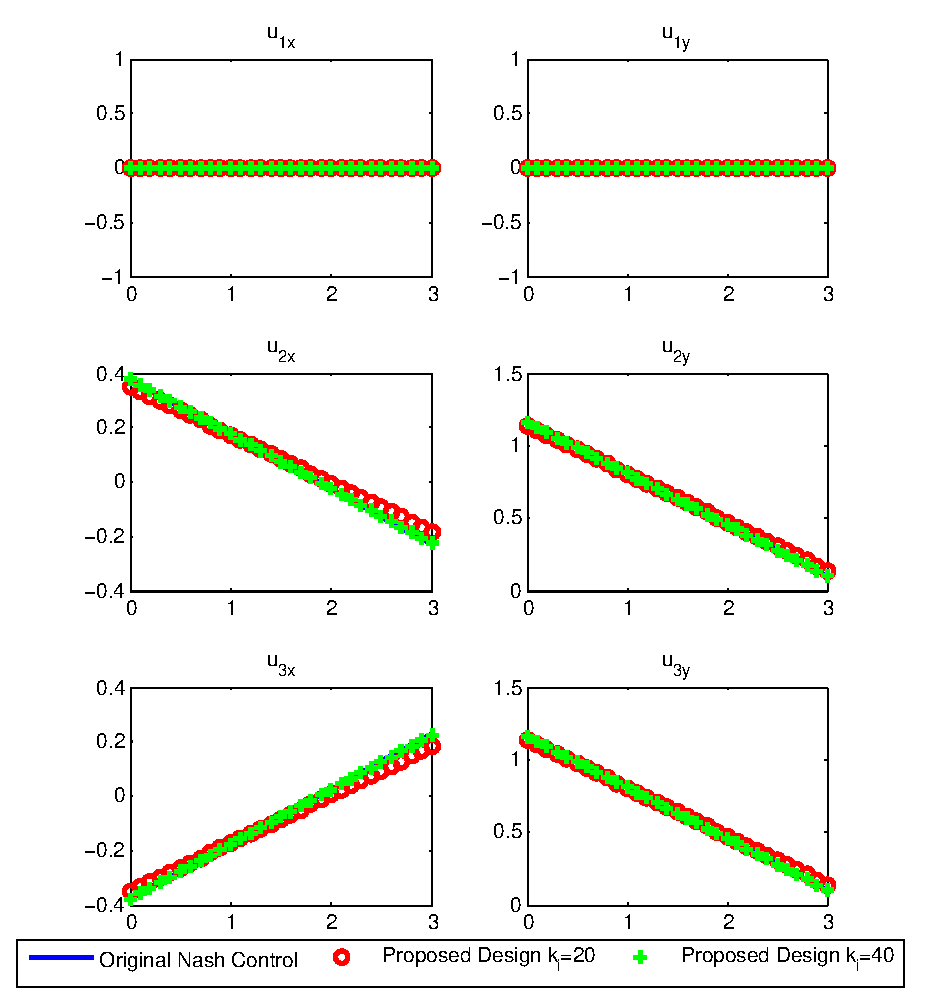
\includegraphics[scale=0.58]{Original_Distributed_control.eps}
      \caption{Nash and proposed designed strategies}\label{Original_Distributed_control}
\end{figure}
The motion trajectories under various control inputs are shown in Figure \ref{TrajectoryUndirected}.
\begin{figure}[h]
      \centering
      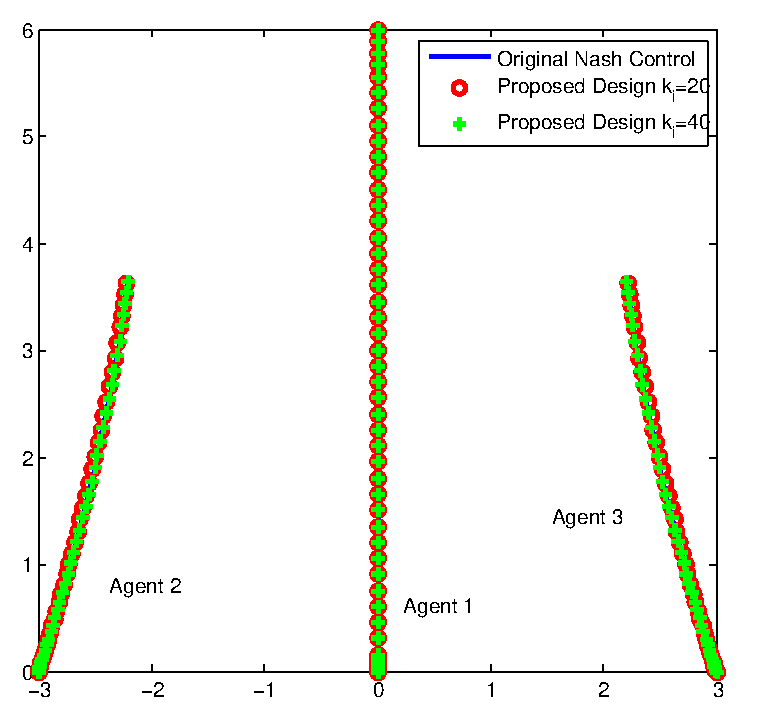
\includegraphics[scale=0.5]{TrajectoryUndirected.eps}
      \caption{Motion trajectories under different control strategies}\label{TrajectoryUndirected}
\end{figure}
Graphically, there does not exist much difference between the trajectories under the original Nash strategies and the ones under designed strategies. Quantitatively, we are able to calculate the total terminal formation error with respect to the desired displaced among the agents, which is
\begin{equation}
\eta=\sum^3_{i=1}\|s_1(t_f)-s_i(t_f)-{\mu_{1i}}\|,
\end{equation}
where $s_i(t_f)$ is agent $i$'s terminal position vector under certain control strategies. Therefore, the total terminal formation errors based on different values of $r_1=r_2=r_3=r$ and $k_1=k_2=k_3=k$ can be summarized into Table \ref{Comparison}.
\begin{table}[h]\normalsize
\centering
\begin{tabular}{|l|c|c|c|}
  \hline
  % after \\: \hline or \cline{col1-col2} \cline{col3-col4} ...
         & Nash & $k=20$ & $k=40$ \\
         \hline
         $\eta\;\;(r=0.2)$ & 0.2162 & 0.2177 & 0.2162 \\
         \hline
  $\eta\;\;(r=1)$ &  0.8164 &  0.8513 & 0.8179 \\
  \hline
  $\eta\;\;(r=5)$ &  2.6541 & 2.6920 & 2.6560 \\
  \hline
\end{tabular}
\caption{Total terminal formation errors in Scenario 1}\label{Comparison}
\end{table}
From the table, it is clear to see that the total terminal formation error decreases as $k_i$ increase because as mentioned, larger $k_i$ will result in more accurate terminal state estimates and more accurate control inputs (with respect to the Nash strategies). It is also clear to see that the total terminal formation error increases as $r$ increases. This is because that if agents put higher penalties on the control effort or energy (i.e., the quadratic term of the control input in (\ref{JiFormation})), they will try to reduce more on control energy instead of the terminal formation errors in order to minimize their performance indices in (\ref{JiFormation}) during the time period of the formation control. Based on more simulation data, the relationship among $\eta$, $k$, and $r$ can be depicted in Figure \ref{Relationship}.
\begin{figure}[h]
      \centering
      \includegraphics[scale=0.5]{PlotT.eps}
      \caption{Relationship among $\eta$, $r$, and $k$}\label{Relationship}
\end{figure}
As we can see in the figure, when $r$ is small, the variance of the total terminal formation error $\eta$ among different $k$ is small, and when $r$ is large, the variance of the total terminal formation error $\eta$ among different $k$ becomes large. Another application of Figure \ref{Relationship} is to determine the lowest update gain $k$ needs to achieve a desired terminal formation error. For instance, if we want to determine a update gain that can achieve a maximum terminal formation error of 2 given $r=2$, then we can find that a value of $k$ less than $6$ is good choice from the figure. Therefore, this figure provides a intuitive way of choosing a proper update gain, especially to avoid choosing a high gain which is undesired in many real life applications.

\textbf{Scenario 2}: We now consider the scenario where there are three agents with undirected communication topology as shown in Figure \ref{Formation3undirected}.
\begin{figure}[h]
      \centering
      \includegraphics[scale=0.8]{Formation3undirected.eps}
      \caption{Three agents with undirected graph}\label{Formation3undirected}
\end{figure}
With this communication topology, both Nash and Pareto strategies can be derived. The initial states of the agents and the performance index parameters are the same as the ones in Scenario 1. For both Nash strategy design and Pareto strategy design, the gain $k_i$ in the terminal state estimation equation (\ref{update}) and (\ref{updatehphv}) are set equal to $40$ for all $i=1,2,3$. For the Pareto strategies, the convex parameters in (\ref{convexcombination}) are set to be $\alpha_1=\alpha_2=\alpha_3=1/3$. The Laplacian matrix for the noncooperative in (\ref{laplacian}) and the one for the cooperative case in (\ref{laplacianFormation}) are
\[\mathcal{L}=\begin{bmatrix}
2&-1&-1\\
-1&1&0\\
-1&0&1
\end{bmatrix}\quad\mbox{and}\quad \mathcal{L}=\begin{bmatrix}
\frac{4}{3}&-\frac{2}{3}&-\frac{2}{3}\\
-\frac{2}{3}&\frac{2}{3}&0\\
-\frac{2}{3}&0&\frac{2}{3}
\end{bmatrix},\]
respectively. The resulting motion trajectories under both Nash and Pareto strategies are shown in Figure \ref{NashPareto}.
\begin{figure}[h!]
      \centering
      \includegraphics[scale=0.5]{NashPareto.eps}
      \caption{Motion trajectories under Nash and Pareto strategies}
      \label{NashPareto}
\end{figure}
The total terminal formation errors under different choices of the convex parameters are summarized in Table \ref{Scenario2Table}.
\begin{table}[h]\normalsize
\centering
\begin{tabular}{|c|c|}
  \hline
  % after \\: \hline or \cline{col1-col2} \cline{col3-col4} ...
       & $\eta$  \\
       \hline
  Nash & 0.4856  \\
  \hline
  Pareto ($\alpha_1=\alpha_2=\alpha_3=1/3$)&0.3033\\
  \hline
  Pareto ($\alpha_1=1/6,\alpha_2=2/3,\alpha_3=1/6$)&0.3128\\
  \hline
  Pareto ($\alpha_1=2/3,\alpha_2=1/6,\alpha_3=1/6$)&0.1791\\
  \hline
  Pareto ($\alpha_1=0.9,\alpha_2=0.05,\alpha_3=0.05$)&0.0602\\
  \hline
\end{tabular}
\caption{Total terminal formation errors in Scenario 2}\label{Scenario2Table}
\end{table}
As we can clearly see in the table, the agents can actually achieve lower formation error using Pareto strategies than using Nash strategies. This is because the agents are assumed to cooperate with each other in the Pareto optimality. Also note that as we place more weight on agent $1$'s performance index, the total formation error can be reduced. This is because it is much easier to move agent 1 alone to form the desired formation {instead} of moving all the three agents together.
%%%%%%%%%%%%%%%%%%%%%%%%%%%%%%%%%%%%%%%%%%%%%%%%%%%%%%%%%%%%%%%%%%%%%%%%%%%%%%%%

\section{Conclusion}\label{conclusion}
{This paper considers the design of open-loop Nash and Pareto strategies for multi-agent formation control problems. The proposed approach utilizes the distributed estimation of the terminal state variables among the agents through network-based information exchange. The convergence rate of the terminal state estimation algorithm is determined by a scalar gain and can be made sufficiently fast to get a better approximation of the real Nash and Pareto strategies. An illustrative example is solved with two scenarios and various comparisons have been made.}

%\addtolength{\textheight}{-12cm}% This command serves to balance the column lengths
                                  % on the last page of the document manually. It shortens
                                  % the textheight of the last page by a suitable amount.
                                  % This command does not take effect until the next page
                                  % so it should come on the page before the last. Make
                                  % sure that you do not shorten the textheight too much.

%%%%%%%%%%%%%%%%%%%%%%%%%%%%%%%%%%%%%%%%%%%%%%%%%%%%%%%%%%%%%%%%%%%%%%%%%%%%%%%%



%%%%%%%%%%%%%%%%%%%%%%%%%%%%%%%%%%%%%%%%%%%%%%%%%%%%%%%%%%%%%%%%%%%%%%%%%%%%%%%%



%%%%%%%%%%%%%%%%%%%%%%%%%%%%%%%%%%%%%%%%%%%%%%%%%%%%%%%%%%%%%%%%%%%%%%%%%%%%%%%%
%\section*{APPENDIX}
%\subsection{Proof of Theorem \ref{Nash1}}
%\begin{proof}
%%For the evader, since it only observes pursuers $1$ to $n_p$, the pursuit-evasion game in the evader's perspective is between it and these pursuers. Therefore,
%Based on the system dynamics (\ref{zidot}) and performance indices (\ref{J0}) and (\ref{Jp1}), we define the following Hamiltonians:
%\begin{align*}
%&H_0=\frac{r_0}{2}\|u_0\|^2  +\sum^{n_p}_{j=1} \lambda_{0j}^T(B_0u_0-B_pu_j)\\
%&H_i=\frac{r_p}{2}\|u_i\|^2  +\lambda_{i}^T(B_0u_0-B_pu_i)\quad \quad
%\forall i=1,\cdots,n_p\\
%&H_i=\frac{r_c}{2}\|u_i\|^2  +\lambda_{i}^T(B_0u_0-B_pu_i)\quad\quad\forall i=(n_p+1),\cdots,N,
%\end{align*}
%where vectors $\lambda_{0j}$ and $\lambda_i$ are the Lagrangian multipliers. Since the second-order Hessian matrix of Hamiltonian $H_i$ with respect to $u_i$ is positive definite for all $i=0,1,\cdots,n_p$, the following necessary conditions according to the Pontryagin's minimum principle \cite{pontreiiagin1962mathematical} are also sufficient for the Nash equilibrium:
%\begin{subequations}
%\begin{align}
%&\dot{\lambda}_{0i}=\dot{\lambda}_i =-\frac{\partial H_0}{\partial z_i}=-\frac{\partial H_i}{\partial z_i}=0\quad \forall i=1,\cdots,N,\label{lambdaconstant}\\
%&\lambda_{0i}(t_f)=-f_0z_i(t_f),\quad \forall i=1,\cdots,N,\label{nec2}\\
%&\lambda_i(t_f)=\left\{\begin{array}{ll}
%f_p z_i(t_f)&i=1,\cdots,n_p\\
%f_c\sum_{\{i,j\}\in\mathcal{E}} [z_i(t_f)-z_j(t_f)]&i=(n_p+1),\cdots,N\\
%\end{array}\right.\label{Nec2},\\
%&0=\frac{\partial H_0}{\partial u_0}=r_0u_0+ B_0^T\sum^{n_p}_{j=1}\lambda_{0j}, \label{nec3}\\
%&0=\frac{\partial H_i}{\partial u_i}=
%\left\{\begin{array}{ll}
%r_pu_i+B_p^T\lambda_i&i=1,\cdots,n_p\\
%r_cu_i-B_p^T\lambda_i&i=(n_p+1),\cdots,N\\
%\end{array}\right..\label{nec4}
%\end{align}
%\end{subequations}
%From conditions (\ref{lambdaconstant}), vectors $\lambda_{0i}$ and $\lambda_i$ are constant and equal to the terminal conditions (\ref{nec2}) and (\ref{Nec2}). Substituting $\lambda_{0i}$ and $\lambda_{i}$ into (\ref{nec3})-(\ref{nec4}) yields
%\begin{subequations}\label{globalNashTerminal}
%\begin{align}
%&u_0=\frac{f_0}{r_0} B^T_0\sum^{n_p}_{j=1}z_j(t_f), \label{u0NashTerminal}\\
%&u_i= \frac{f_p}{r_p}B^T_pz_i(t_f) \quad\quad\forall i=1,\cdots,n_p£¬ \label{uiNashTerminal}
%\end{align}
%\end{subequations}
%and (\ref{uinoENash2}). Substituting (\ref{globalNashTerminal}) to (\ref{zidot}) and integrating the equation from $0$ to $t_f$ yield
%\begin{align}
%(I+S_p)z_i(t_f) =&z_i(0)+S_0\sum^{n_p}_{j=1}z_j(t_f). \label{difference}
%\end{align}
%where where matrices $S_0$ and $S_p$ are defined in (\ref{S}). Summing up the above equation for all $i=1,\cdots,n_p$ yields
%\begin{equation}
%\sum^{n_p}_{j=1}z_j(t_f) =M_0\sum^{n_p}_{j=1}z_j(0)\label{zjtf}
%\end{equation}
%provided that matrix $M_0$ in (\ref{M}) exists. Substituting (\ref{zjtf}) into (\ref{globalNashTerminal}) yields (\ref{u0Nash}) and (\ref{uiNash}).
%\end{proof}







%
%Appendixes should appear before the acknowledgment.

%\section*{ACKNOWLEDGMENT}


\bibliographystyle{IEEEtran}
\bibliography{Mybib}




\end{document}
